\chapter{实验及结果}
\label{cha:6-experiment}
  
  实验对比一章依然分为图像着色与视频着色分别讨论。

\section{黑白图像着色}
\label{sec:6-image-color}

  对于图像着色,本文在三个数据集上进行了实验,与两种目前效果最好的学习算法进行了对比。

  三个数据集分别是:LSUN-CHURCH~\cite{DBLP:journals/corr/YuZSSX15},是一个教堂图片的数据集,数据规模为12w训练集,300验证集;CIFAR-10~\cite{CIFAR-10},是一个包含10类图片的数据集,数据规模为5w训练集,1w测试集;IMAGE-NET~\cite{DBLP:journals/ijcv/RussakovskyDSKS15},是一个大型的分类数据集,包含1000类物体,本文采用了它的部分子集,数据规模为28w训练集,1w测试集。

  进行对比的两个图像自动着色算法是Iizuka等人Siggraph2016的\inlinecite{IizukaSIGGRAPH2016},与Zhang等人ECCV2016的\inlinecite{zhang2016colorful}。

  本文选择均方误差(MSE)作为评价标准,即以网络着色结果与真是彩色图像之间的像素均方差作为误差。表~\ref{tab:6-image-error}给出了误差对比。需要注意的是,本文的网络是在三个数据集下分别独立的,即Ours$_l$指的是在LSUN-CHURCH下训练的本文的网络,Ours$_c$与Ours$_i$以此类推;另外,均方误差值取的是64x64分辨率图片的像素误差和,且像素UV值已归一化到[-1,1]。

  \begin{table}[H]
    \centering
    \begin{minipage}[t]{0.8\linewidth}
    \caption{黑白图像着色均方误差对比}
    \label{tab:6-image-error}
      \begin{tabularx}{\linewidth}{|l|X|X|X|}
        \hline
        \multirow{2}*{\diagbox[width=6em]{\heiti 方法}{\heiti 数据集}} & \multirow{2}*{LSUN-CHURCH} & \multirow{2}*{CIFAR-10} & \multirow{2}*{IMAGE-NET} \\
         & & & \\\hline
        Ours$_l$ & 127.1 & - & - \\\hline
        Ours$_c$ & - & 347.9 & - \\\hline
        Ours$_i$ & - & - & 174.5 \\\hline
        Zhang    & 151.8 & 367.5 & 282.8 \\\hline
        Iizuka   & \textbf{86.7}  & \textbf{117.2} & \textbf{127.6} \\\hline
      \end{tabularx}
    \end{minipage}
  \end{table}

  从表~\ref{tab:6-image-error}进行方法的纵向对比,可以发现本文的生成对抗模型总体来说表现比Zhang~\cite{zhang2016colorful}等人的卷积神经网络好,但与Iizuka~\cite{IizukaSIGGRAPH2016}等人的卷积神经网络相比还差距较大;在本文的方法内部进行数据集间的横向对比可以发现:当在只有一类物体的LSUN-CHURCH数据集上时,本文的均方误差较小,当在物体种类较多的IMAGE-NET上训练时,误差变大;当图像分辨率变小时(CIFAR-10的图像分辨率只有32x32),误差也会明显增大。

  图~\ref{fig:lsun-compare},图~\ref{fig:cifar-compare},图~\ref{fig:imagenet-compare}分别给出了LSUN-CHURCH、CIFAR-10、IMAGE-NET数据集下本文的网络着色与真实图像的对比。

  \begin{figure}[ht]
    \centering
    \subcaptionbox{本文网络的着色结果\label{fig:lsun_fake}}
      {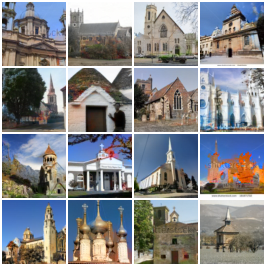
\includegraphics[width=0.3\paperwidth]{lsun_fake}}
    \hspace{2em}
    \subcaptionbox{真实彩色图像\label{fig:lsun_real}}
        {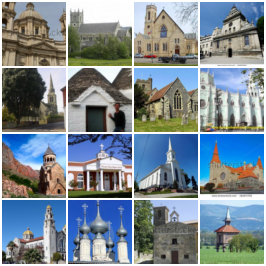
\includegraphics[width=0.3\paperwidth]{lsun_real}}
    \caption{LSUN-CHURCH数据集测试结果}
    \label{fig:lsun-compare}
  \end{figure}

  \begin{figure}[ht]
    \centering
    \subcaptionbox{本文网络的着色结果\label{fig:cifar_fake}}
      {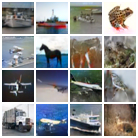
\includegraphics[width=0.3\paperwidth]{cifar_fake}}
    \hspace{2em}
    \subcaptionbox{真实彩色图像\label{fig:cifar_real}}
        {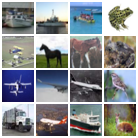
\includegraphics[width=0.3\paperwidth]{cifar_real}}
    \caption{CIFAR-10数据集测试结果}
    \label{fig:cifar-compare}
  \end{figure}

  \begin{figure}[ht]
    \centering
    \subcaptionbox{本文网络的着色结果\label{fig:imagenet_fake}}
      {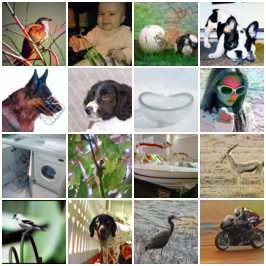
\includegraphics[width=0.3\paperwidth]{imagenet_fake}}
    \hspace{2em}
    \subcaptionbox{真实彩色图像\label{fig:imagenet_real}}
        {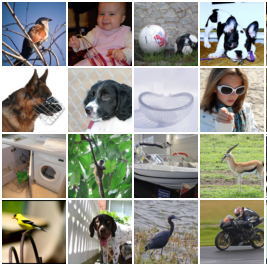
\includegraphics[width=0.3\paperwidth]{imagenet_real}}
    \caption{IMAGE-NET数据集测试结果}
    \label{fig:imagenet-compare}
  \end{figure}

  从这些结果中分析得出这样的结论:GAN处理着色问题相比CNN更逊色。图像风格转换的任务已经被证明非常适合GAN模型,Zhu~\cite{DBLP:journals/corr/ZhuPIE17}等人最新的网络结构cycleGAN在做两种风格图片转换的任务上取得了很好的效果,比如油画风格与照片写实风格之间的互相转换。着色问题也可以看作一个风格转换问题(黑白风格到彩色风格的转换),但相比前者,着色问题里图像的域更大:前者可能只是莫奈的油画风格与真实照片的转换,而着色中的图像包含了多种物体的多种可能颜色,对于一种物体有效的着色对于另一种物体就不行。所以在单一物体的LSUN-CHURCH数据集上表现更好,而在多物体的CIFAR-10与IMAGE-NET的数据集上就表现更差。

\section{黑白视频着色}
\label{sec:6-video-color}

  对于视频着色,本文在UCF11数据集上进行了实验,没有现有的自动着色算法可比较。

  UCF11~\cite{DBLP:conf/cvpr/LiuLS09}是一个人体动作识别的数据库,包含11类人类不同运动的短视频共2000段。在这个数据集上使用本文第~\ref{cha:4-video-color}章中的3D模型时,生成器无法向真实图像进行学习,结果是着色的关键帧一直是非常暗淡没有什么色彩,在反复调试后也不能得到有意义的结果,图~\ref{fig:3d_result}就是本文的3D网络着色结果。于是只好暂时放弃用3D模型着色的想法,使用2D的GAN模型给关键帧着色。

  \begin{figure}[H]
    \centering
    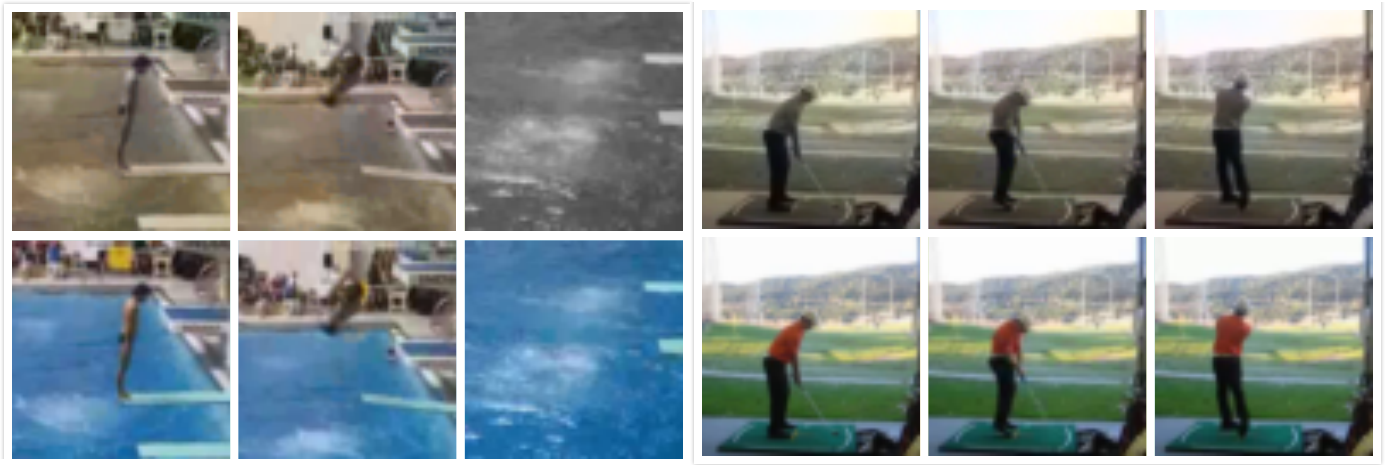
\includegraphics[width=0.7\paperwidth]{3d_result}
    \caption[3D网络着色结果]{3D网络的着色结果。第一行是本文的着色,第二行是真实视频帧;前三列来自一个跳水视频,后三列来自一个高尔夫视频}
    \label{fig:3d_result}
  \end{figure}

  使用2D网络对视频着色的流程在第~\ref{cha:5-other-algorithm}章已经介绍过了。训练时本文使用UCF11中的2000个视频,每个视频等间距取采样帧作为训练图像数据,共约2w的训练集,另外有100个视频留作测试集。

  图~\ref{fig:2d_result}是本文的2D网络着色结果。

  \begin{figure}[H]
    \centering
    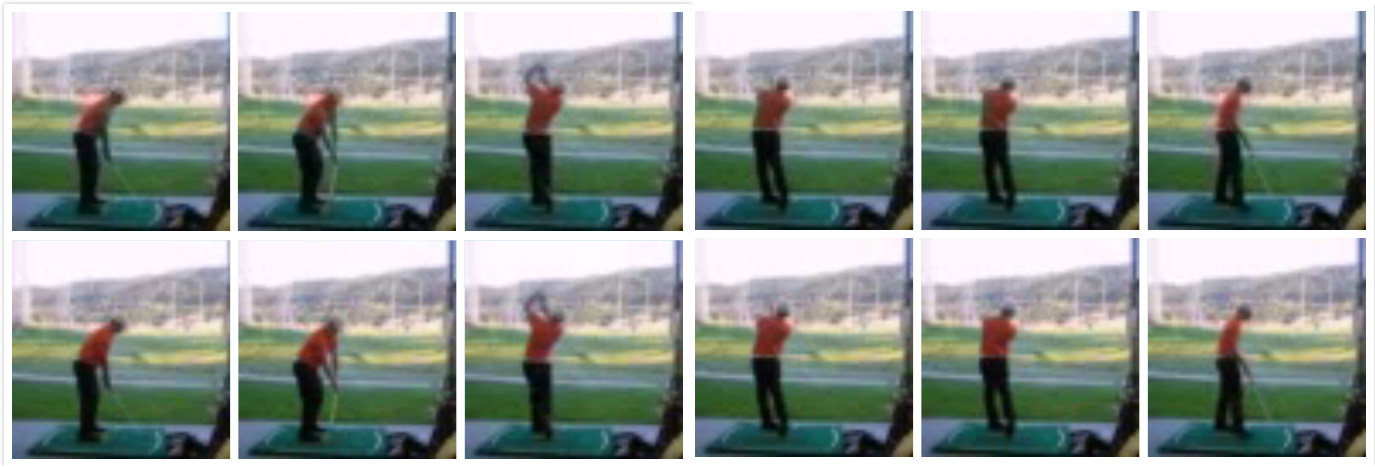
\includegraphics[width=0.7\paperwidth]{2d_result}
    \caption[2D网络着色结果]{3D网络的着色结果。第一行是我们的着色视频帧,第二行是真实视频帧}
    \label{fig:2d_result}
  \end{figure}

  另外单帧着色带来的时间空间不稳定性通过本文第~\ref{cha:5-other-algorithm}章中的平滑可以解决,这一点可以从图~\ref{fig:2d_result_compare}中看出。

  \begin{figure}[H]
    \centering
    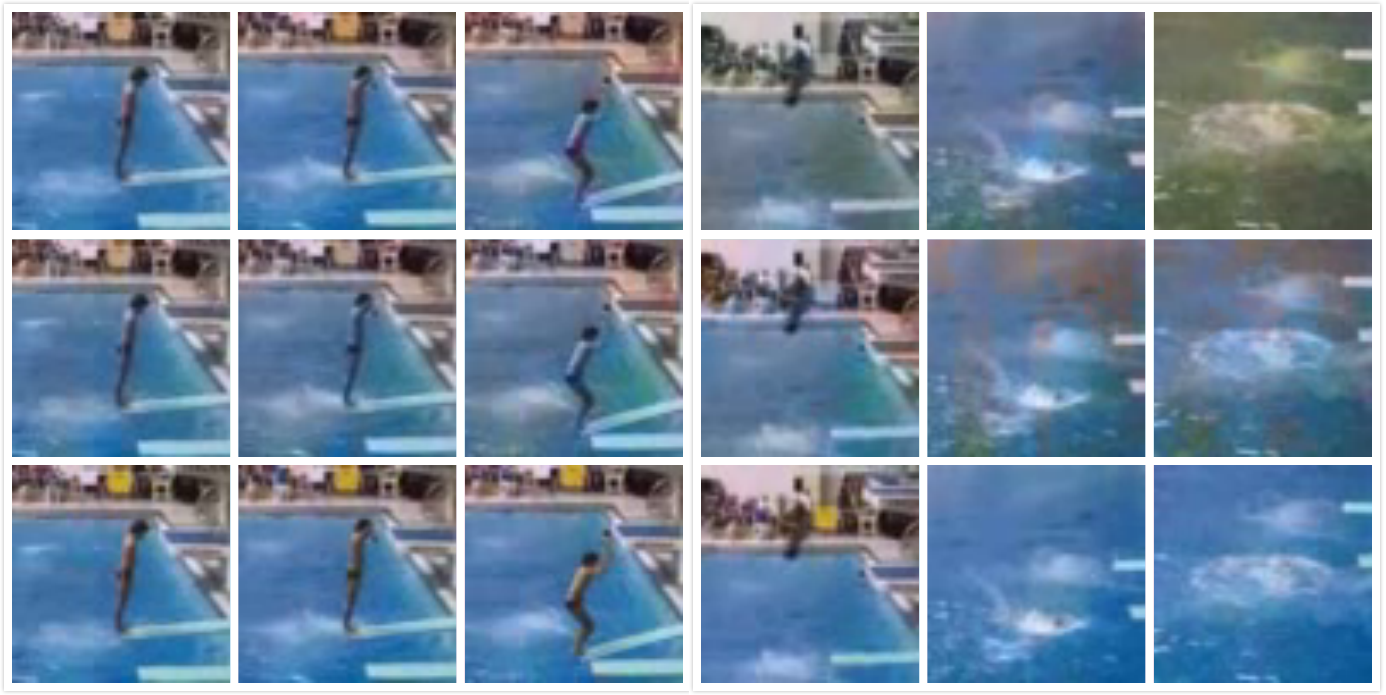
\includegraphics[width=0.7\paperwidth]{2d_result_compare}
    \caption[时空平滑效果比较]{时空平滑效果比较。第一行是本文直接使用2D网络对每一帧着色的结果,第二行是本文用2D网络对关键帧着色然后进行时空平滑处理的结果,第三行是真实视频帧}
    \label{fig:2d_result_compare}
  \end{figure}

  另外本文也用图像着色中LSUN-CHURCH教堂数据集训练的网络给大礼堂进行了着色,如图~\ref{fig:extra_result}。

  \begin{figure}[H]
    \centering
    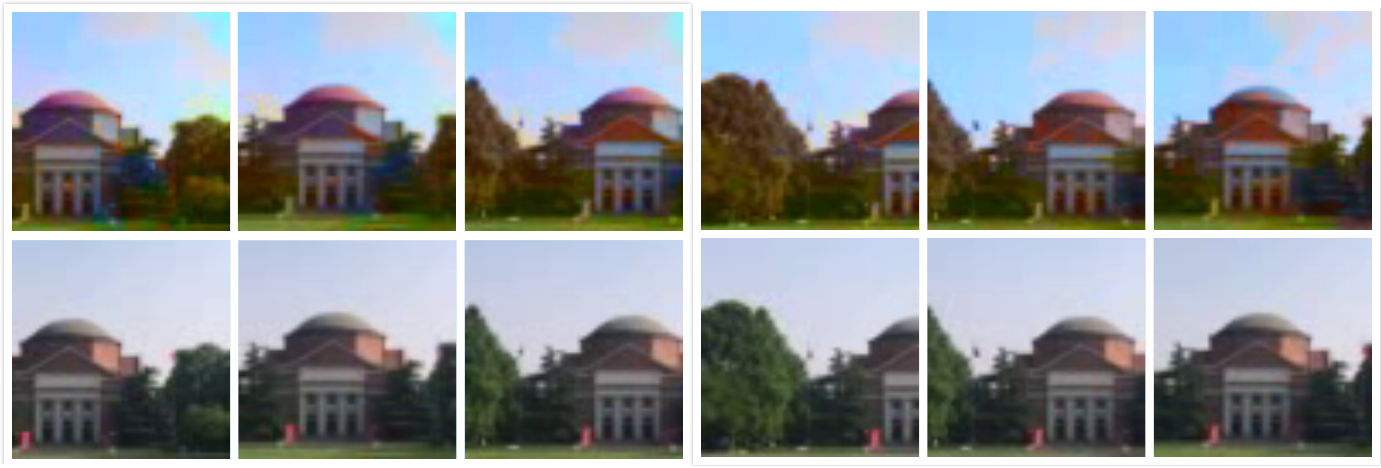
\includegraphics[width=0.7\paperwidth]{extra_result}
    \caption[大礼堂着色效果]{大礼堂着色效果。第一行是本文的着色结果,第二是真实拍摄的视频}
    \label{fig:extra_result}
  \end{figure}

  \begin{figure}[H]
    \centering
    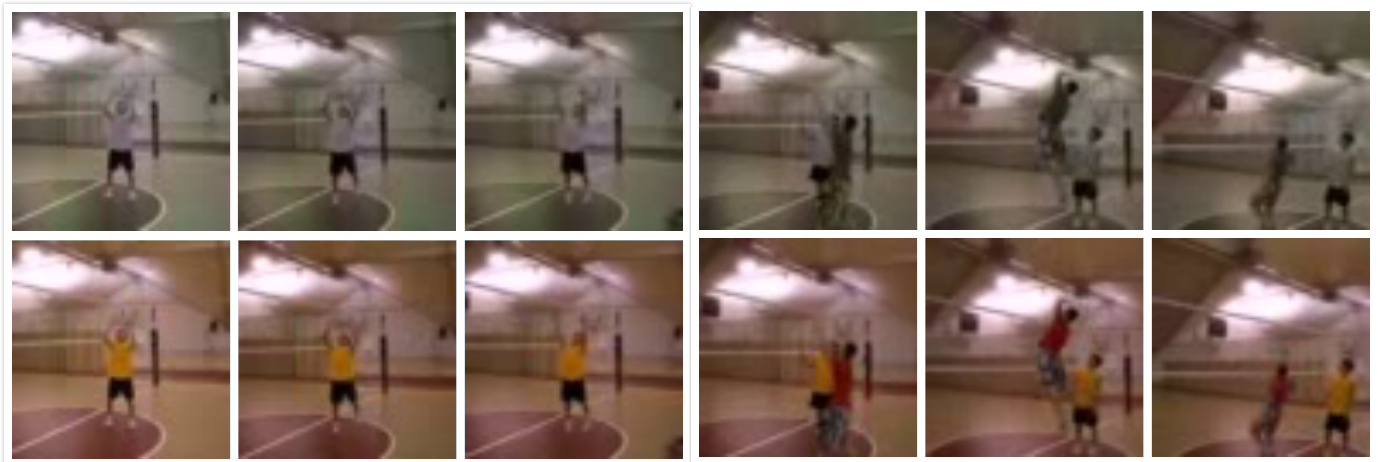
\includegraphics[width=0.7\paperwidth]{failure_case}
    \caption[失败案例]{失败案例。第一行是本文的着色结果,第二是真实拍摄的视频}
    \label{fig:failure_case}
  \end{figure}  

  不过在UCF11数据集下也有一些失败的案例,如图~\ref{fig:failure_case},通常的体现是没有什么色彩。分析原因为:当视频场景中物体动作幅度不是很大时,着色能有较好的效果(如高尔夫击球),相反动作幅度较大时(如排球扣球),网络便不那么稳定;场景的特征颜色较明显时(如跳水中的蓝色),着色结果很理想,而场景没有明显的颜色特征时,网络变只能给出灰褐色的平凡结果。





  